% 0L  
\vspace*{\fill}

\begin{figure}[h!]
    \centering
    \begin{subfigure}[b]{\textwidth}
        \centering
        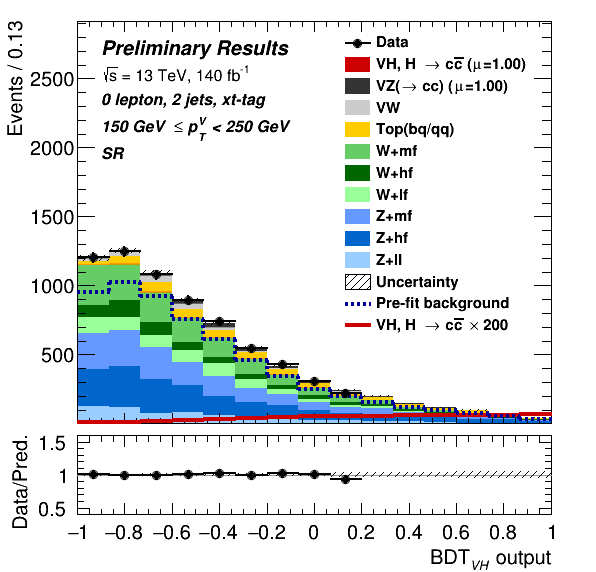
\includegraphics[width=0.32\textwidth]{Images/VH/Own_fit/postfit_VHcc/Region_distmva_BMax250_BMin150_DSR_J2_TTypext_T2_L0_Y6051_GlobalFit_conditionnal_mu1.png}
        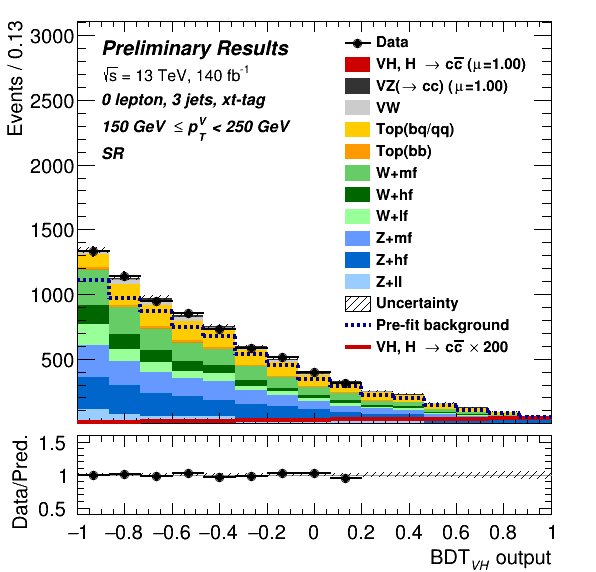
\includegraphics[width=0.32\textwidth]{Images/VH/Own_fit/postfit_VHcc/Region_distmva_BMax250_BMin150_DSR_J3_TTypext_T2_L0_Y6051_GlobalFit_conditionnal_mu1.png}
        \caption{150 < \ptv\ < 250 GeV.}
        \label{fig:plots_VHcc_OL_150_SR_2c}
    \end{subfigure}
    \begin{subfigure}[b]{\textwidth}
        \centering
        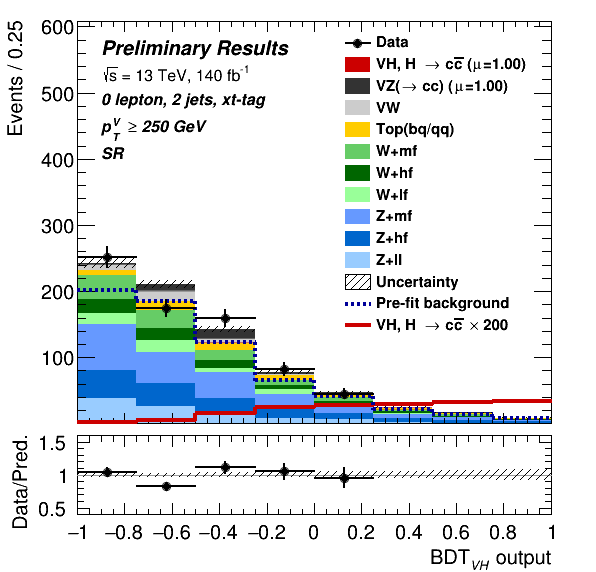
\includegraphics[width=0.32\textwidth]{Images/VH/Own_fit/postfit_VHcc/Region_distmva_BMin250_DSR_J2_TTypext_T2_L0_Y6051_GlobalFit_conditionnal_mu1.png}
        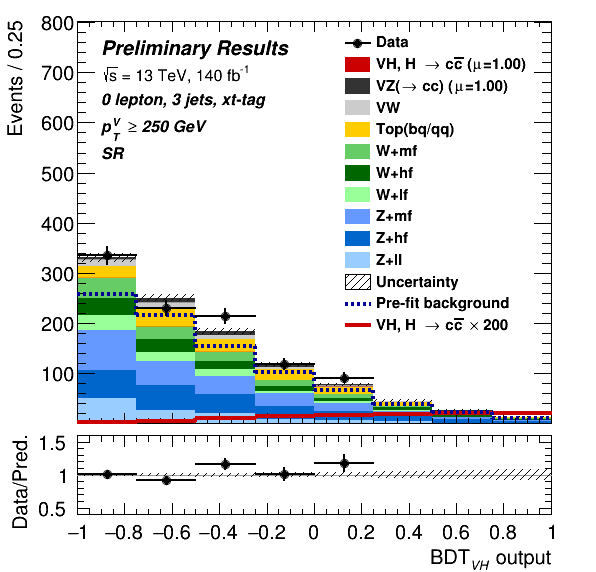
\includegraphics[width=0.32\textwidth]{Images/VH/Own_fit/postfit_VHcc/Region_distmva_BMin250_DSR_J3_TTypext_T2_L0_Y6051_GlobalFit_conditionnal_mu1.png}
        \caption{250 GeV < \ptv.}
        \label{fig:plots_VHcc_OL_250_SR_2c}
    \end{subfigure}
    \caption{\gls{bdt} distributions in the 0L 2 $c$-tagged signal regions, 2-jet (left) and 3-jet (right).}
    \label{fig:plots_VHcc_OL_SR_2c}
\end{figure} 
\begin{figure}[h!]
    \centering
    \begin{subfigure}[b]{\textwidth}
        \centering
        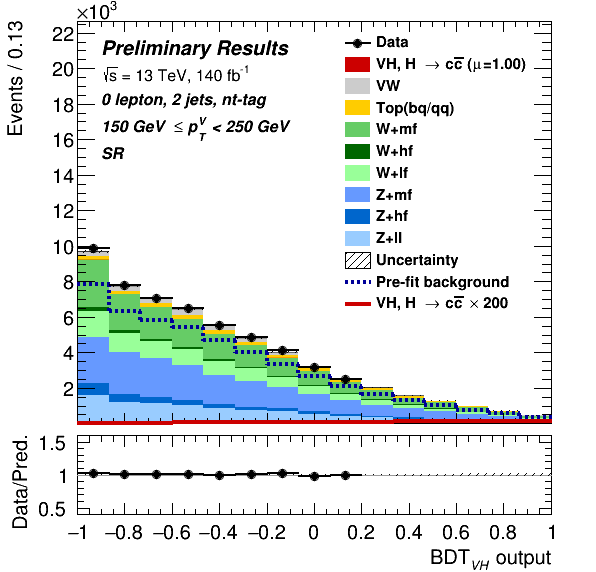
\includegraphics[width=0.32\textwidth]{Images/VH/Own_fit/postfit_VHcc/Region_distmva_BMax250_BMin150_DSR_J2_TTypent_T1_L0_Y6051_GlobalFit_conditionnal_mu1.png}
        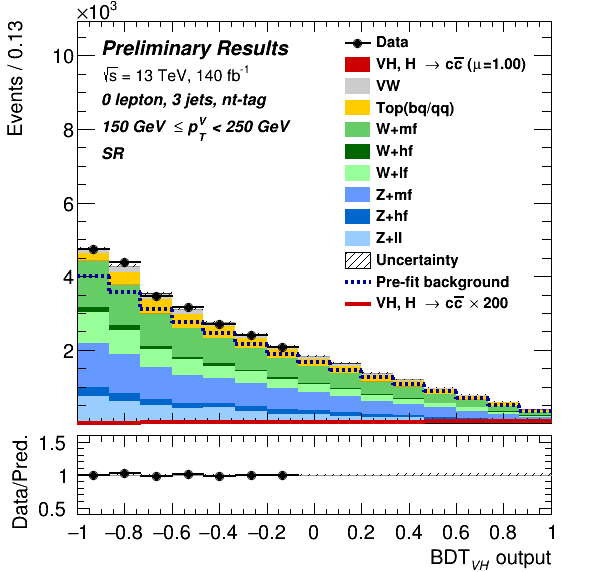
\includegraphics[width=0.32\textwidth]{Images/VH/Own_fit/postfit_VHcc/Region_distmva_BMax250_BMin150_DSR_J3_TTypent_T1_L0_Y6051_GlobalFit_conditionnal_mu1.png}
        \caption{150 < \ptv\ < 250 GeV.}
        \label{fig:plots_VHcc_OL_150_SR_1c}
    \end{subfigure}
    \begin{subfigure}[b]{\textwidth}
        \centering
        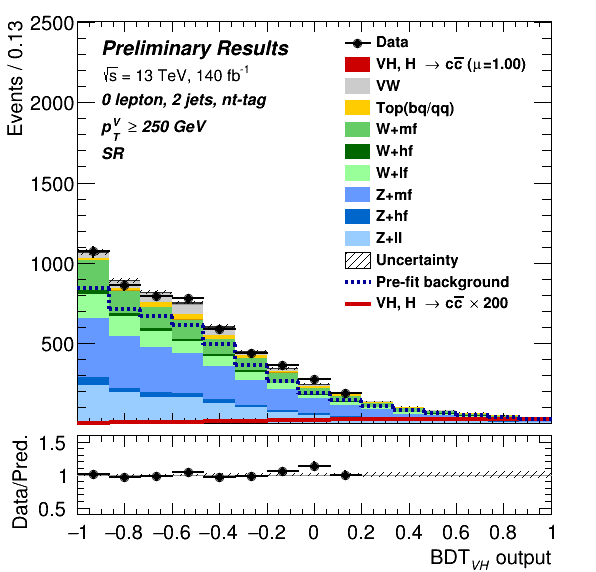
\includegraphics[width=0.32\textwidth]{Images/VH/Own_fit/postfit_VHcc/Region_distmva_BMin250_DSR_J2_TTypent_T1_L0_Y6051_GlobalFit_conditionnal_mu1.png}
        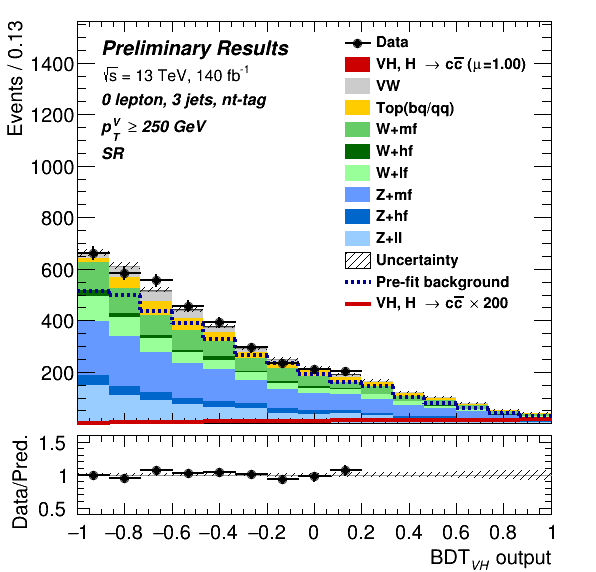
\includegraphics[width=0.32\textwidth]{Images/VH/Own_fit/postfit_VHcc/Region_distmva_BMin250_DSR_J3_TTypent_T1_L0_Y6051_GlobalFit_conditionnal_mu1.png}
        \caption{250 GeV < \ptv.}
        \label{fig:plots_VHcc_OL_250_SR_1c}
    \end{subfigure}
    \caption{\gls{bdt} distributions in the 0L 1 $c$-tagged signal regions, 2-jet (left) and 3-jet (right).}
    \label{fig:plots_VHcc_OL_SR_1c}
\end{figure} 

\vspace*{\fill} 

\begin{figure}[h!]
    \centering
    \begin{subfigure}[b]{\textwidth}
        \centering
        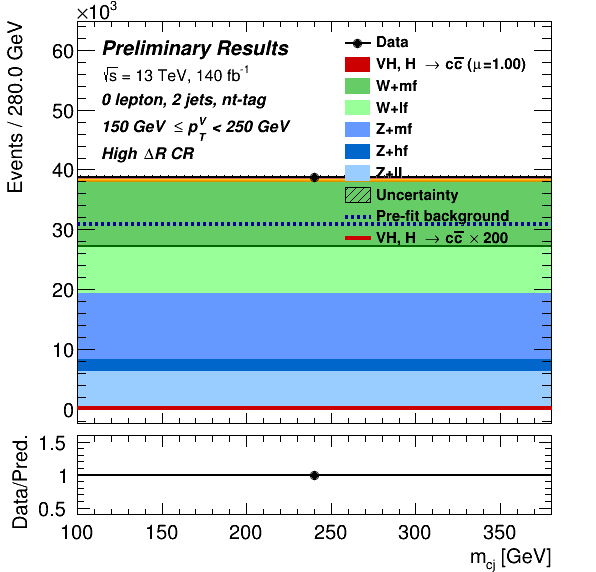
\includegraphics[width=0.32\textwidth]{Images/VH/Own_fit/postfit_VHcc/Region_distmBB_BMax250_BMin150_DCRHigh_J2_TTypent_T1_L0_Y6051_GlobalFit_conditionnal_mu1.png}
        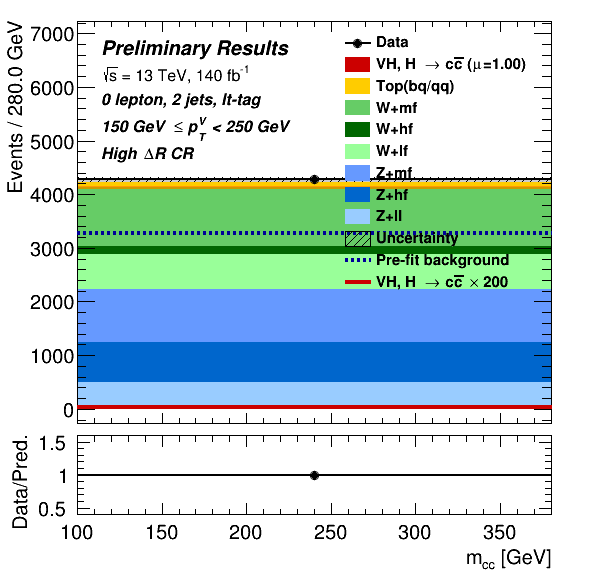
\includegraphics[width=0.32\textwidth]{Images/VH/Own_fit/postfit_VHcc/Region_distmBB_BMax250_BMin150_DCRHigh_J2_TTypelt_T2_L0_Y6051_GlobalFit_conditionnal_mu1.png}
        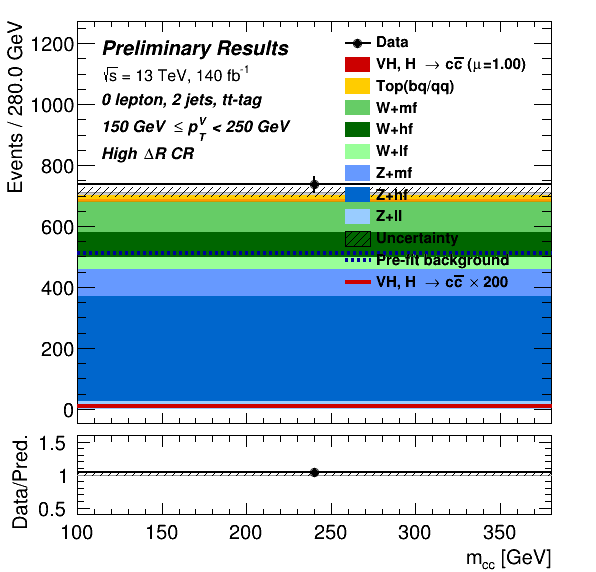
\includegraphics[width=0.32\textwidth]{Images/VH/Own_fit/postfit_VHcc/Region_distmBB_BMax250_BMin150_DCRHigh_J2_TTypett_T2_L0_Y6051_GlobalFit_conditionnal_mu1.png}
        \caption{150 < \ptv\ < 250 GeV, $TN$- (left), $LT$- (centre), and $TT$-tag (right).}
        \label{fig:plots_VHcc_OL_150_CRH_2c_2J}
    \end{subfigure}
    \begin{subfigure}[b]{\textwidth}
        \centering
        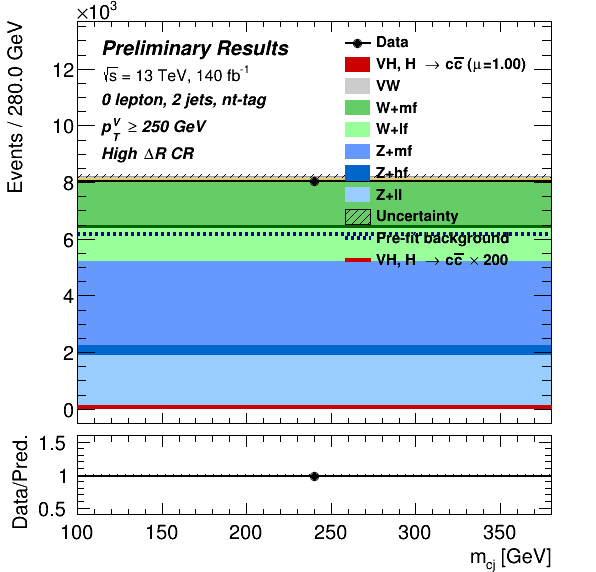
\includegraphics[width=0.32\textwidth]{Images/VH/Own_fit/postfit_VHcc/Region_distmBB_BMin250_DCRHigh_J2_TTypent_T1_L0_Y6051_GlobalFit_conditionnal_mu1.png}
        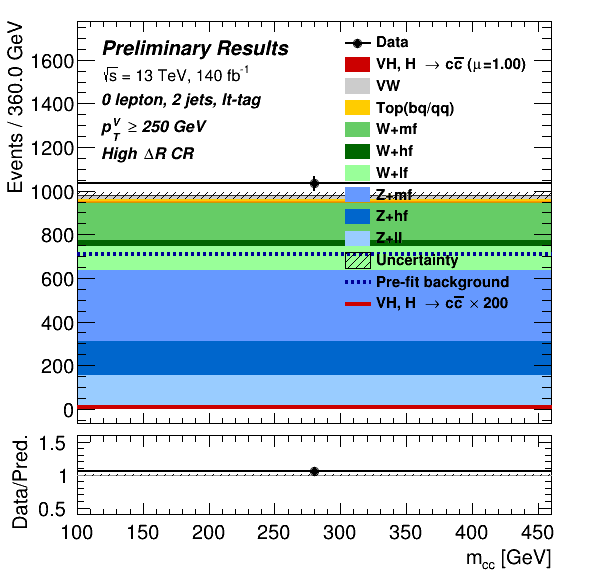
\includegraphics[width=0.32\textwidth]{Images/VH/Own_fit/postfit_VHcc/Region_distmBB_BMin250_DCRHigh_J2_TTypelt_T2_L0_Y6051_GlobalFit_conditionnal_mu1.png}
        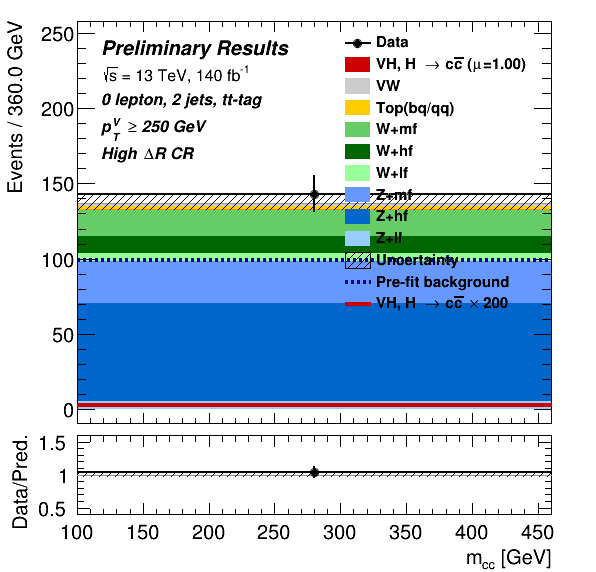
\includegraphics[width=0.32\textwidth]{Images/VH/Own_fit/postfit_VHcc/Region_distmBB_BMin250_DCRHigh_J2_TTypett_T2_L0_Y6051_GlobalFit_conditionnal_mu1.png}
        \caption{250 GeV < \ptv, $TN$- (left), $LT$- (centre), and $TT$-tag (right).}
        \label{fig:plots_VHcc_OL_250_CRH_2c_2J}
    \end{subfigure}
    \caption{$H$-candidate mass distributions in the 0L 2-jet \highdr\ CRs.}
    \label{fig:plots_VHcc_OL_CRH_2c_2J}
\end{figure} 
\begin{figure}[h!]
    \centering
    \begin{subfigure}[b]{\textwidth}
        \centering
        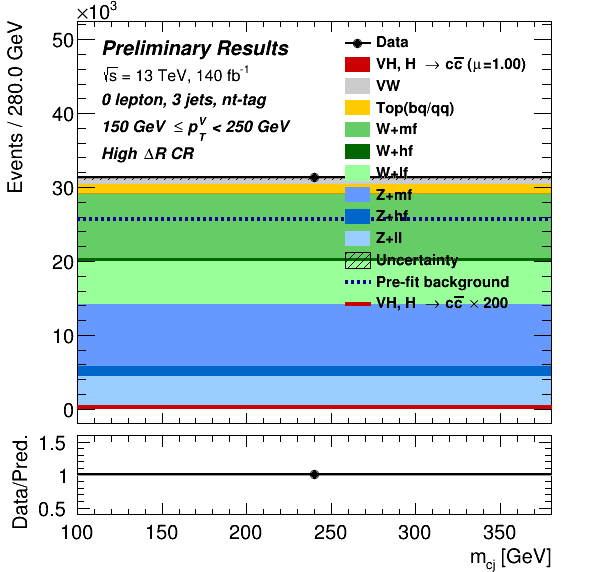
\includegraphics[width=0.32\textwidth]{Images/VH/Own_fit/postfit_VHcc/Region_distmBB_BMax250_BMin150_DCRHigh_J3_TTypent_T1_L0_Y6051_GlobalFit_conditionnal_mu1.png}
        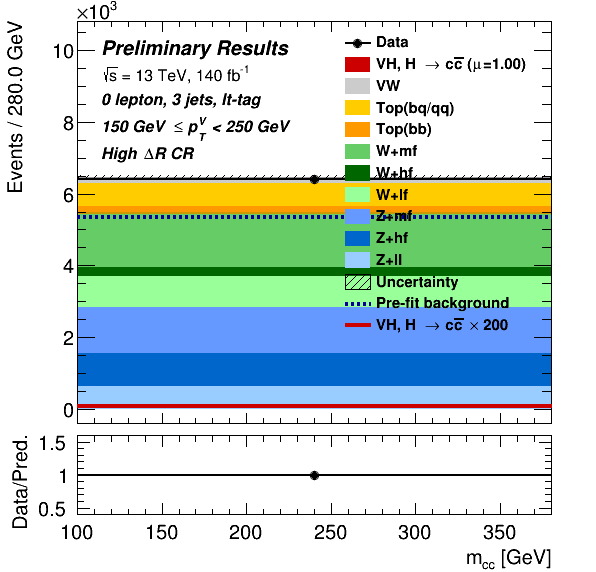
\includegraphics[width=0.32\textwidth]{Images/VH/Own_fit/postfit_VHcc/Region_distmBB_BMax250_BMin150_DCRHigh_J3_TTypelt_T2_L0_Y6051_GlobalFit_conditionnal_mu1.png}
        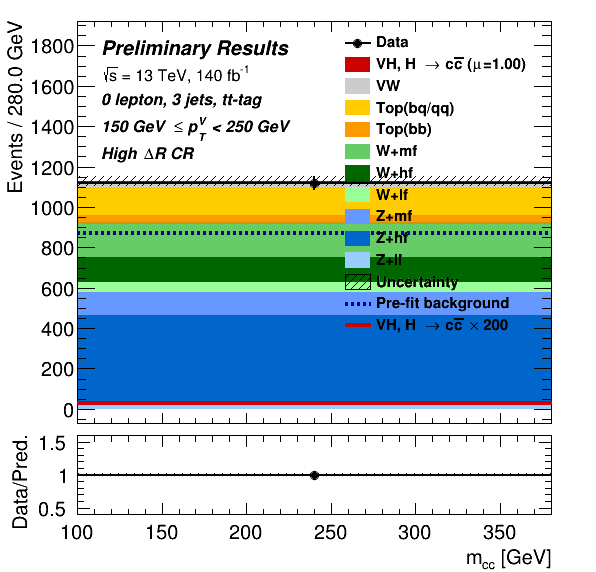
\includegraphics[width=0.32\textwidth]{Images/VH/Own_fit/postfit_VHcc/Region_distmBB_BMax250_BMin150_DCRHigh_J3_TTypett_T2_L0_Y6051_GlobalFit_conditionnal_mu1.png}
        \caption{150 GeV < \ptv\ < 250 GeV, $TN$- (left), $LT$- (centre), and $TT$-tag (right).}
        \label{fig:plots_VHcc_OL_150_CRH_2c_3J}
    \end{subfigure}
    \begin{subfigure}[b]{\textwidth}
        \centering

        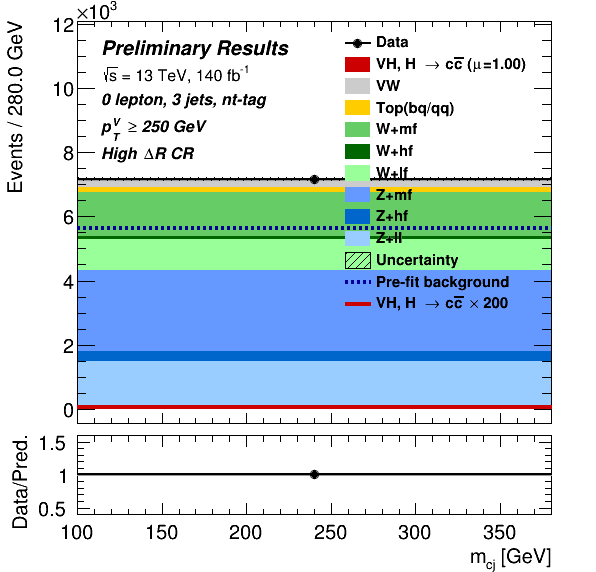
\includegraphics[width=0.32\textwidth]{Images/VH/Own_fit/postfit_VHcc/Region_distmBB_BMin250_DCRHigh_J3_TTypent_T1_L0_Y6051_GlobalFit_conditionnal_mu1.png}
        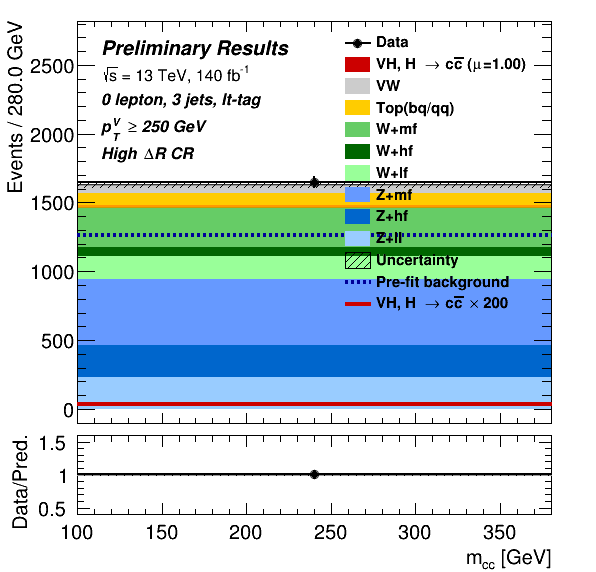
\includegraphics[width=0.32\textwidth]{Images/VH/Own_fit/postfit_VHcc/Region_distmBB_BMin250_DCRHigh_J3_TTypelt_T2_L0_Y6051_GlobalFit_conditionnal_mu1.png}
        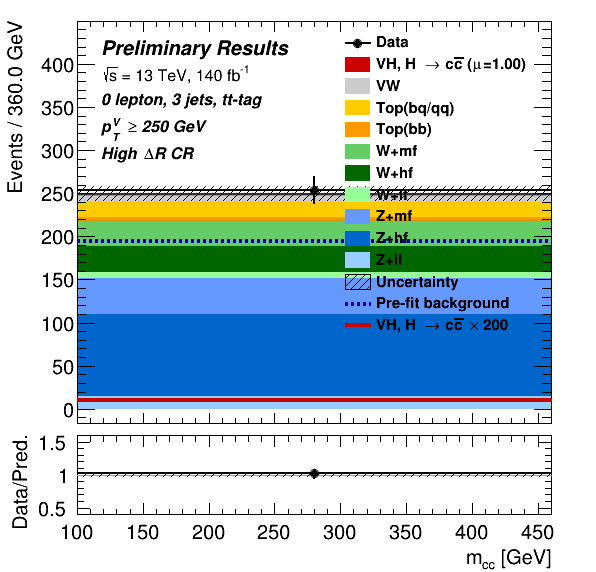
\includegraphics[width=0.32\textwidth]{Images/VH/Own_fit/postfit_VHcc/Region_distmBB_BMin250_DCRHigh_J3_TTypett_T2_L0_Y6051_GlobalFit_conditionnal_mu1.png}
        \caption{250 GeV < \ptv, $TN$- (left), $LT$- (centre), and $TT$-tag (right).}
        \label{fig:plots_VHcc_OL_250_CRH_2c_3J}
    \end{subfigure}
    \caption{$H$-candidate mass distributions in the 0L 3-jet \highdr\ CRs.}
    \label{fig:plots_VHcc_OL_CRH_2c_3J}
\end{figure} 

\vspace*{\fill} 

% TopCR 0L
\begin{figure}[h!]
    \centering
    \begin{subfigure}[b]{\textwidth}
        \centering
        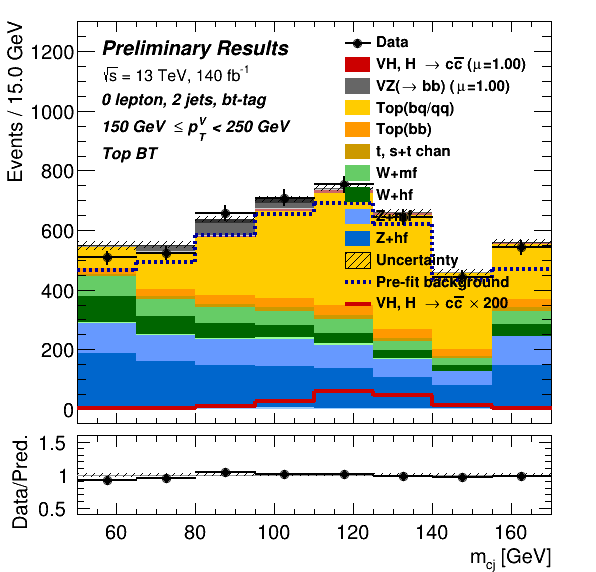
\includegraphics[width=0.32\textwidth]{Images/VH/Own_fit/postfit_VHcc/Region_distmBB_BMax250_BMin150_DtopCRBC_J2_TTypebt_T1_L0_Y6051_GlobalFit_conditionnal_mu1.png}
        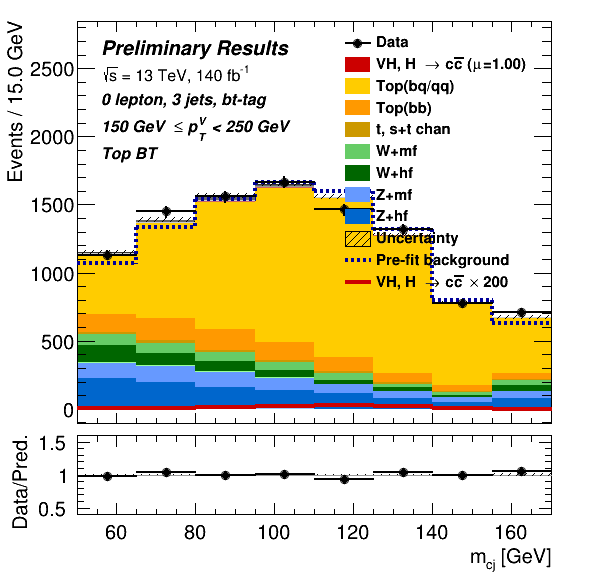
\includegraphics[width=0.32\textwidth]{Images/VH/Own_fit/postfit_VHcc/Region_distmBB_BMax250_BMin150_DtopCRBC_J3_TTypebt_T1_L0_Y6051_GlobalFit_conditionnal_mu1.png}
        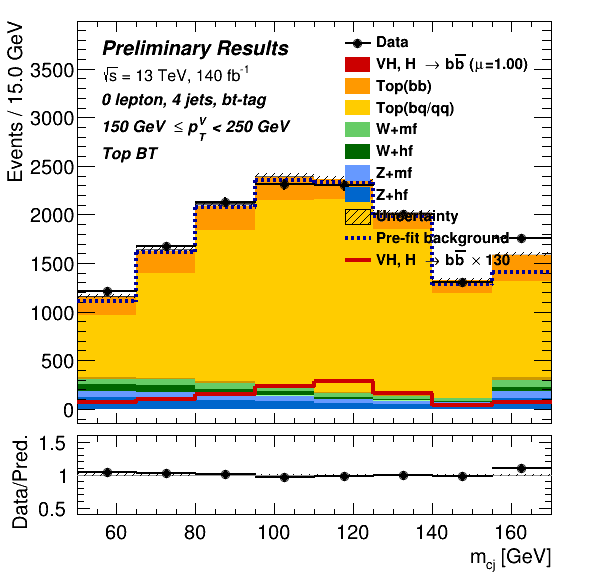
\includegraphics[width=0.32\textwidth]{Images/VH/Own_fit/postfit_VHbb/Region_distmBB_BMax250_BMin150_DtopCRBC_J4_TTypebt_T1_L0_Y6051_GlobalFit_conditionnal_mu1.png} % Must be VHbb due to 4j
        \caption{150 < \ptv\ < 250 GeV.}
        \label{fig:plots_VHcc_OL_150_TopCR_2c}
    \end{subfigure}
    \begin{subfigure}[b]{\textwidth}
        \centering
        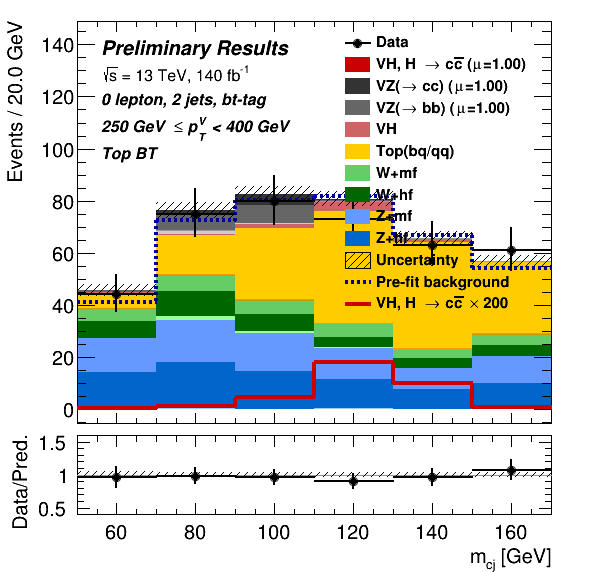
\includegraphics[width=0.32\textwidth]{Images/VH/Own_fit/postfit_VHcc/Region_distmBB_BMax400_BMin250_DtopCRBC_J2_TTypebt_T1_L0_Y6051_GlobalFit_conditionnal_mu1.png}
        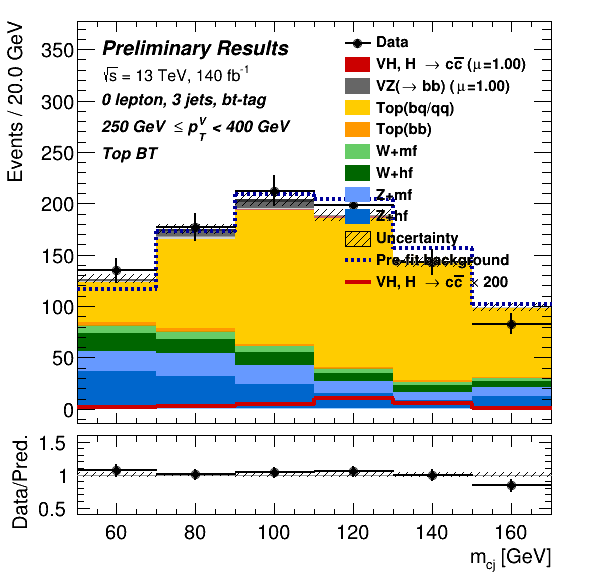
\includegraphics[width=0.32\textwidth]{Images/VH/Own_fit/postfit_VHcc/Region_distmBB_BMax400_BMin250_DtopCRBC_J3_TTypebt_T1_L0_Y6051_GlobalFit_conditionnal_mu1.png}
        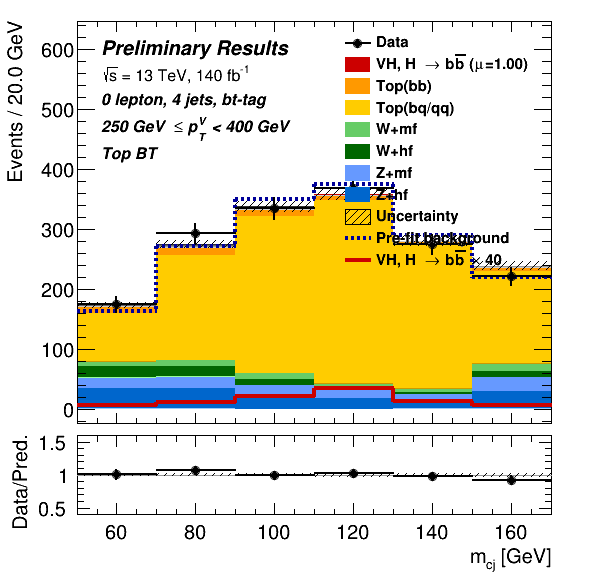
\includegraphics[width=0.32\textwidth]{Images/VH/Own_fit/postfit_VHbb/Region_distmBB_BMax400_BMin250_DtopCRBC_J4_TTypebt_T1_L0_Y6051_GlobalFit_conditionnal_mu1.png} % Must be VHbb due to 4j
        \caption{250 GeV < \ptv\ < 400 GeV.}
        \label{fig:plots_VHcc_OL_250_TopCR_2c}
    \end{subfigure}
    \caption{$H$-candidate mass distributions in the 0L $BT$-tagged Top CRs, 2-jet (left), 3-jet (centre), and 4-jet (right).}
    \label{fig:plots_VHcc_OL_TopCR_2c}
\end{figure} 

\vspace*{\fill} \newpage
\vspace*{\fill} 

% 1L
\begin{figure}[h!]
    \centering
    \begin{subfigure}[b]{\textwidth}
        \centering
        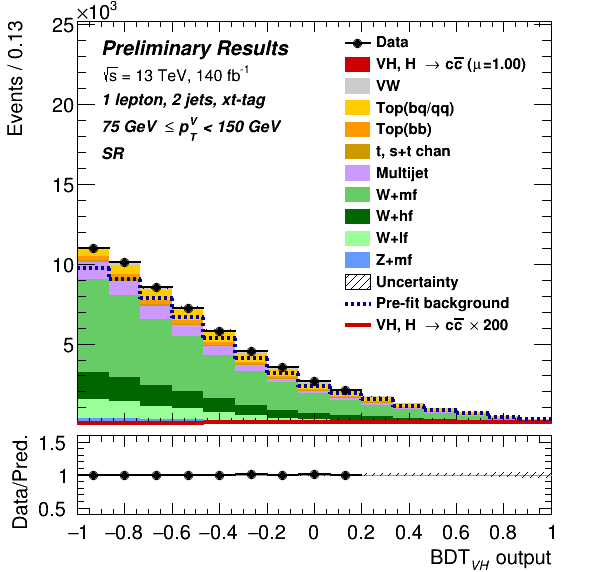
\includegraphics[width=0.32\textwidth]{Images/VH/Own_fit/postfit_VHcc/Region_distmva_BMax150_BMin75_DSR_J2_TTypext_T2_L1_Y6051_GlobalFit_conditionnal_mu1.png}
        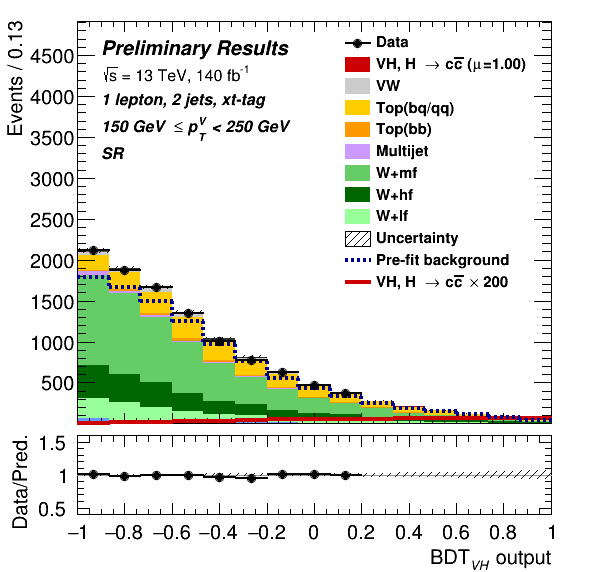
\includegraphics[width=0.32\textwidth]{Images/VH/Own_fit/postfit_VHcc/Region_distmva_BMax250_BMin150_DSR_J2_TTypext_T2_L1_Y6051_GlobalFit_conditionnal_mu1.png}
        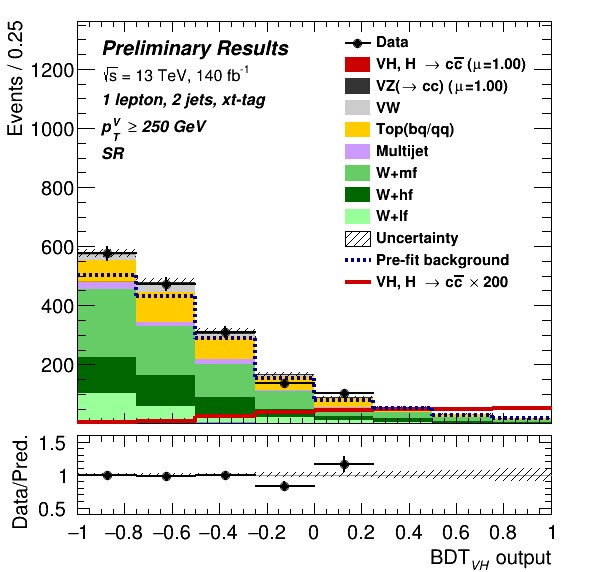
\includegraphics[width=0.32\textwidth]{Images/VH/Own_fit/postfit_VHcc/Region_distmva_BMin250_DSR_J2_TTypext_T2_L1_Y6051_GlobalFit_conditionnal_mu1.png}
        \caption{2-jet, [75, 150] GeV (left), [150, 250] GeV (centre), and 250  GeV $\leq$ (right) \ptv\ regions.}
        \label{fig:plots_VHcc_1L_SR_2J_2c}
    \end{subfigure}
    \begin{subfigure}[b]{\textwidth}
        \centering
        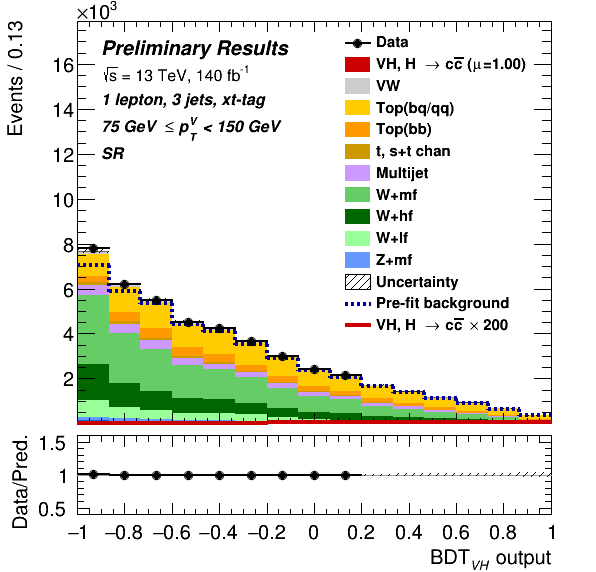
\includegraphics[width=0.32\textwidth]{Images/VH/Own_fit/postfit_VHcc/Region_distmva_BMax150_BMin75_DSR_J3_TTypext_T2_L1_Y6051_GlobalFit_conditionnal_mu1.png}
        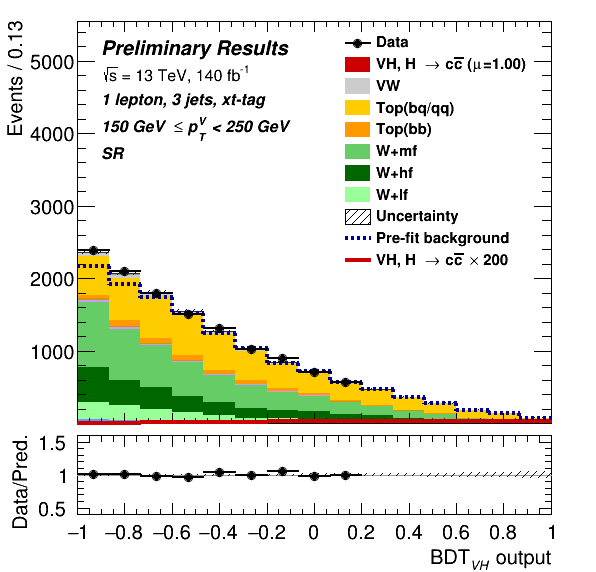
\includegraphics[width=0.32\textwidth]{Images/VH/Own_fit/postfit_VHcc/Region_distmva_BMax250_BMin150_DSR_J3_TTypext_T2_L1_Y6051_GlobalFit_conditionnal_mu1.png}
        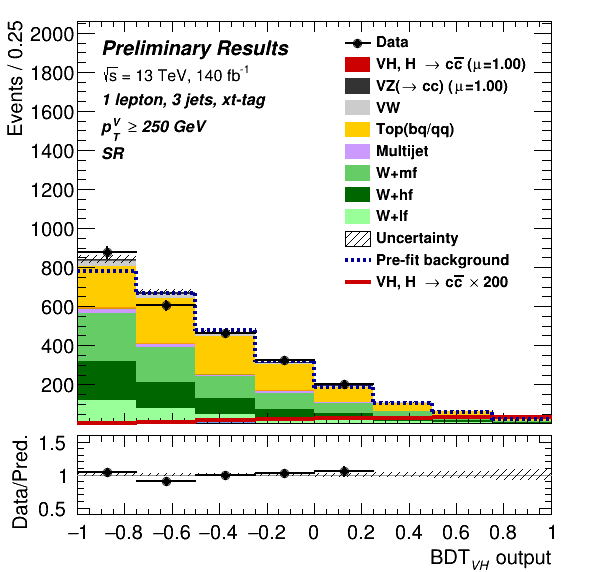
\includegraphics[width=0.32\textwidth]{Images/VH/Own_fit/postfit_VHcc/Region_distmva_BMin250_DSR_J3_TTypext_T2_L1_Y6051_GlobalFit_conditionnal_mu1.png}
        \caption{3-jet, [75, 150] GeV (left), [150, 250] GeV (centre), and 250  GeV $\leq$ (right) \ptv\ regions.}
        \label{fig:plots_VHcc_1L_SR_3J_2c}
    \end{subfigure}
    \caption{\gls{bdt} distributions in the 1L 2 $c$-tagged signal regions.}
    \label{fig:plots_VHcc_1L_SR_2c}
\end{figure}
\begin{figure}[h!]
    \centering
    \begin{subfigure}[b]{\textwidth}
        \centering
        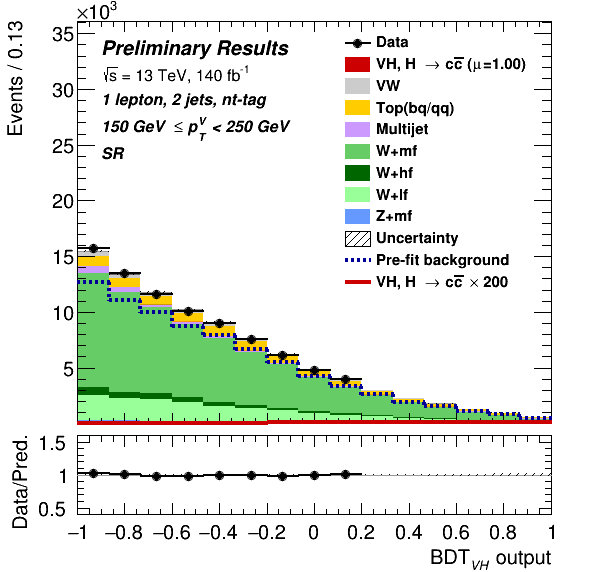
\includegraphics[width=0.32\textwidth]{Images/VH/Own_fit/postfit_VHcc/Region_distmva_BMax250_BMin150_DSR_J2_TTypent_T1_L1_Y6051_GlobalFit_conditionnal_mu1.png}
        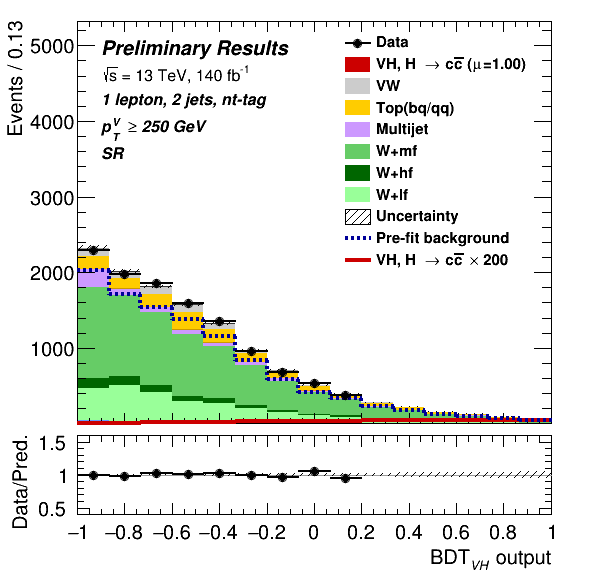
\includegraphics[width=0.32\textwidth]{Images/VH/Own_fit/postfit_VHcc/Region_distmva_BMin250_DSR_J2_TTypent_T1_L1_Y6051_GlobalFit_conditionnal_mu1.png}
        \caption{2-jet, [75, 150] GeV (left), [150, 250] GeV (centre), and 250  GeV $\leq$ (right) \ptv\ regions.}
        \label{fig:plots_VHcc_1L_SR_2J_1c}
    \end{subfigure}
    \begin{subfigure}[b]{\textwidth}
        \centering
        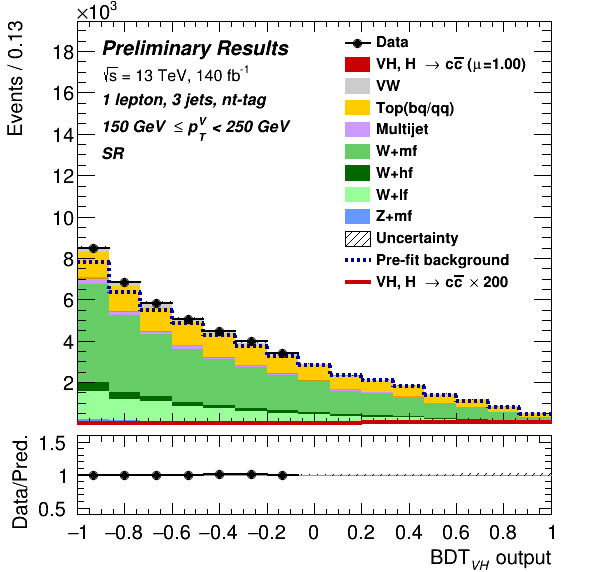
\includegraphics[width=0.32\textwidth]{Images/VH/Own_fit/postfit_VHcc/Region_distmva_BMax250_BMin150_DSR_J3_TTypent_T1_L1_Y6051_GlobalFit_conditionnal_mu1.png}
        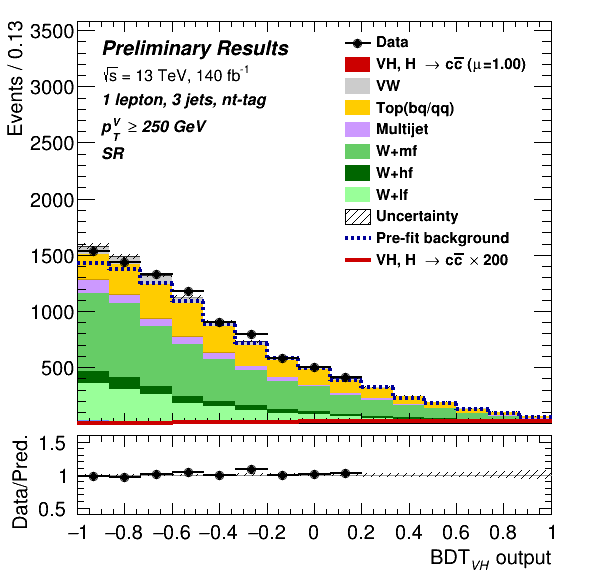
\includegraphics[width=0.32\textwidth]{Images/VH/Own_fit/postfit_VHcc/Region_distmva_BMin250_DSR_J3_TTypent_T1_L1_Y6051_GlobalFit_conditionnal_mu1.png}
        \caption{3-jet, [75, 150] GeV (left), [150, 250] GeV (centre), and 250  GeV $\leq$ (right) \ptv\ regions.}
        \label{fig:plots_VHcc_1L_SR_3J_1c}
    \end{subfigure}
    \caption{\gls{bdt} distributions in the 1L 1 $c$-tagged signal regions.}
    \label{fig:plots_VHcc_1L_SR_1c}
\end{figure}

\newpage
\vspace*{\fill} 


\begin{figure}[h!]
    \centering
    \begin{subfigure}[b]{\textwidth}
        \centering
        
\includegraphics[width=0.32\textwidth]{Images/VH/Own_fit/blank.png}
        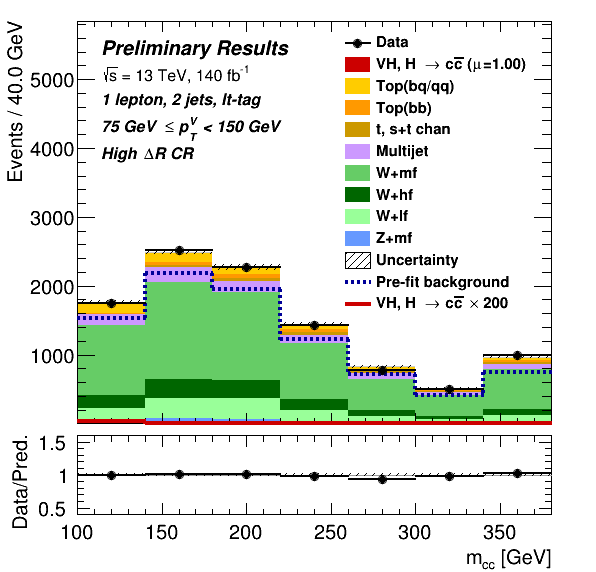
\includegraphics[width=0.32\textwidth]{Images/VH/Own_fit/postfit_VHcc/Region_distmBB_BMax150_BMin75_DCRHigh_J2_TTypelt_T2_L1_Y6051_GlobalFit_conditionnal_mu1.png}
        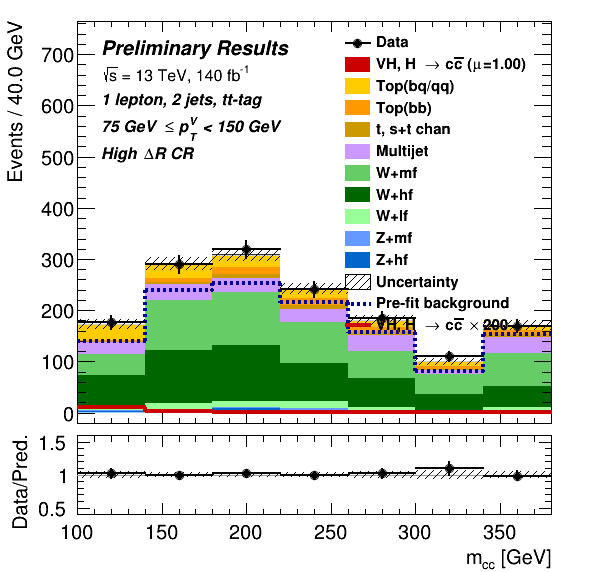
\includegraphics[width=0.32\textwidth]{Images/VH/Own_fit/postfit_VHcc/Region_distmBB_BMax150_BMin75_DCRHigh_J2_TTypett_T2_L1_Y6051_GlobalFit_conditionnal_mu1.png}
        \caption{75 < \ptv\ < 150 GeV ($TN$ not included).}
        \label{fig:plots_VHcc_1L_75_CRH_2J}
    \end{subfigure}
    \begin{subfigure}[b]{\textwidth}
        \centering
        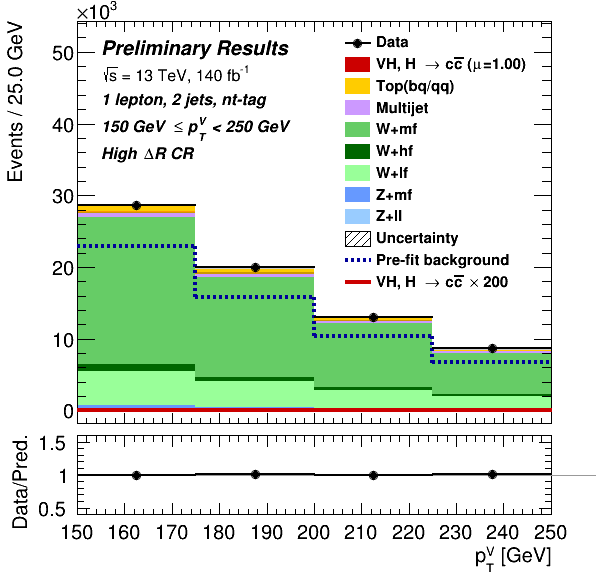
\includegraphics[width=0.32\textwidth]{Images/VH/Own_fit/postfit_VHcc/Region_distpTV_BMax250_BMin150_DCRHigh_J2_TTypent_T1_L1_Y6051_GlobalFit_conditionnal_mu1.png}
        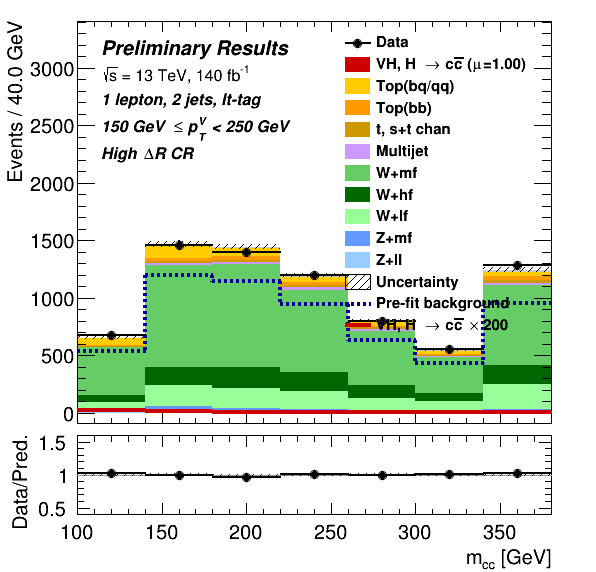
\includegraphics[width=0.32\textwidth]{Images/VH/Own_fit/postfit_VHcc/Region_distmBB_BMax250_BMin150_DCRHigh_J2_TTypelt_T2_L1_Y6051_GlobalFit_conditionnal_mu1.png}
        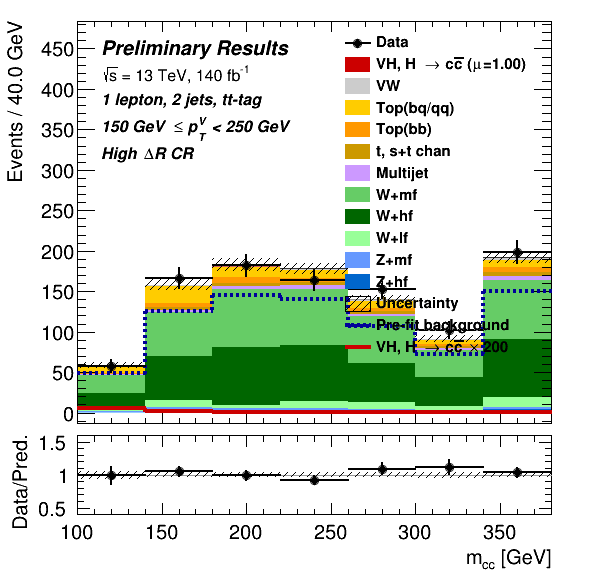
\includegraphics[width=0.32\textwidth]{Images/VH/Own_fit/postfit_VHcc/Region_distmBB_BMax250_BMin150_DCRHigh_J2_TTypett_T2_L1_Y6051_GlobalFit_conditionnal_mu1.png}
        \caption{150 < \ptv\ < 250 GeV.}
        \label{fig:plots_VHcc_1L_150_CRH_2J}
    \end{subfigure}
    \begin{subfigure}[b]{\textwidth}
        \centering
        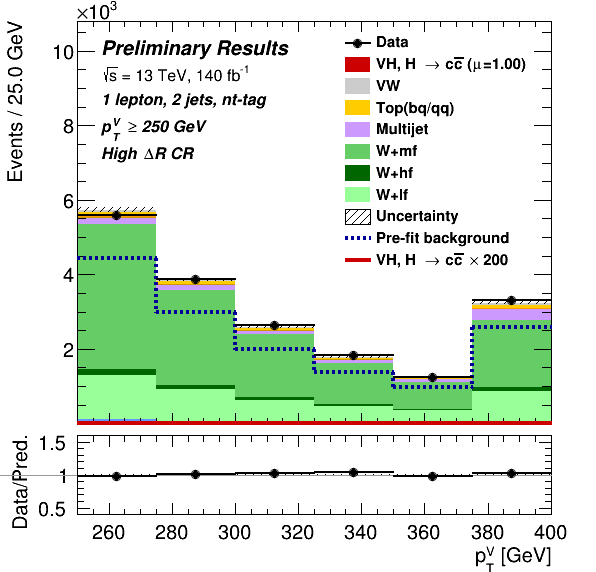
\includegraphics[width=0.32\textwidth]{Images/VH/Own_fit/postfit_VHcc/Region_distpTV_BMin250_DCRHigh_J2_TTypent_T1_L1_Y6051_GlobalFit_conditionnal_mu1.png}
        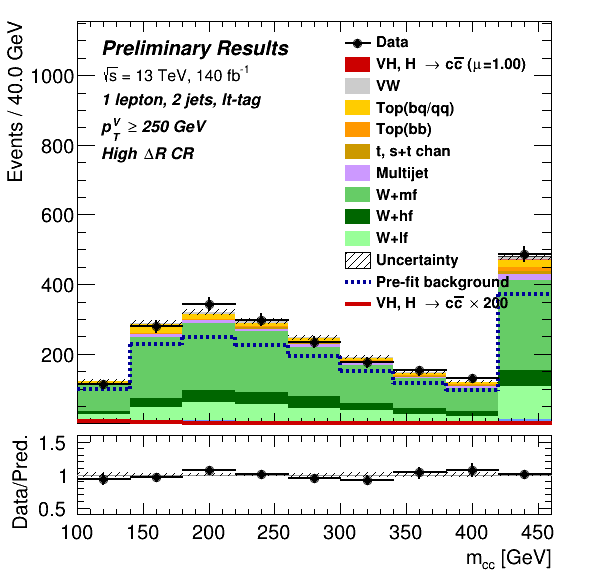
\includegraphics[width=0.32\textwidth]{Images/VH/Own_fit/postfit_VHcc/Region_distmBB_BMin250_DCRHigh_J2_TTypelt_T2_L1_Y6051_GlobalFit_conditionnal_mu1.png}
        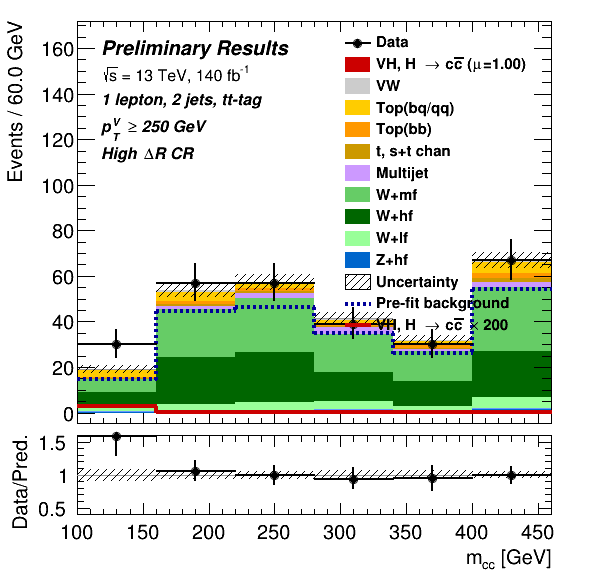
\includegraphics[width=0.32\textwidth]{Images/VH/Own_fit/postfit_VHcc/Region_distmBB_BMin250_DCRHigh_J2_TTypett_T2_L1_Y6051_GlobalFit_conditionnal_mu1.png}
        \caption{250 GeV < \ptv.}
        \label{fig:plots_VHcc_1L_250_CRH_2J}
    \end{subfigure}
    \caption{$TN$-tagged \ptv\ distributions (left) and $LT$- (centre) and $TT$-tagged (right) $H$-candidate mass distributions in the 1L \highdr\ CR 2-jet regions.}
    \label{fig:plots_VHcc_1L_CRH_2J}
\end{figure}

\vspace*{\fill} \newpage
\vspace*{\fill} 

\begin{figure}[h!]
    \centering
    \begin{subfigure}[b]{\textwidth}
        \centering
        
\includegraphics[width=0.32\textwidth]{Images/VH/Own_fit/blank.png}
        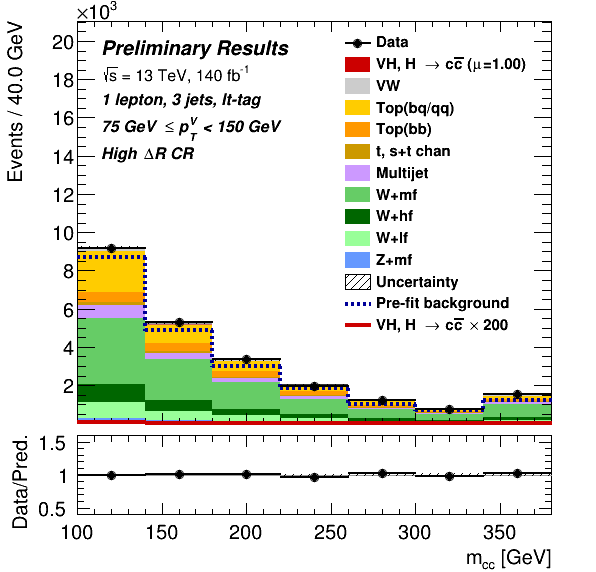
\includegraphics[width=0.32\textwidth]{Images/VH/Own_fit/postfit_VHcc/Region_distmBB_BMax150_BMin75_DCRHigh_J3_TTypelt_T2_L1_Y6051_GlobalFit_conditionnal_mu1.png}
        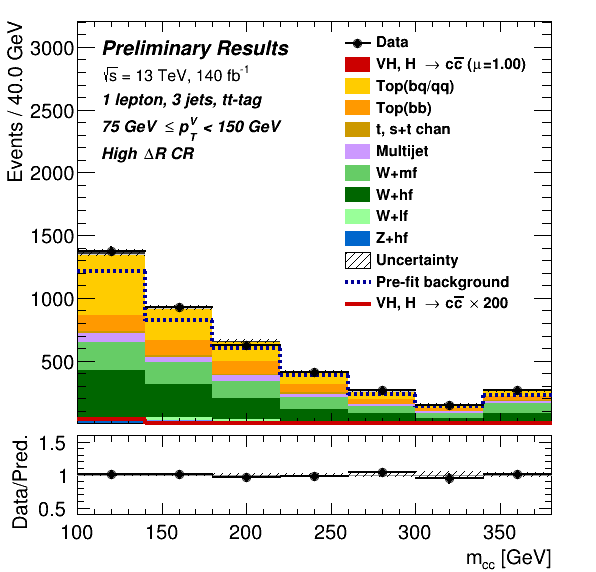
\includegraphics[width=0.32\textwidth]{Images/VH/Own_fit/postfit_VHcc/Region_distmBB_BMax150_BMin75_DCRHigh_J3_TTypett_T2_L1_Y6051_GlobalFit_conditionnal_mu1.png}
        \caption{75 < \ptv\ < 150 GeV ($TN$ not included).}
        \label{fig:plots_VHcc_1L_75_CRH_3J}
    \end{subfigure}
    \begin{subfigure}[b]{\textwidth}
        \centering
        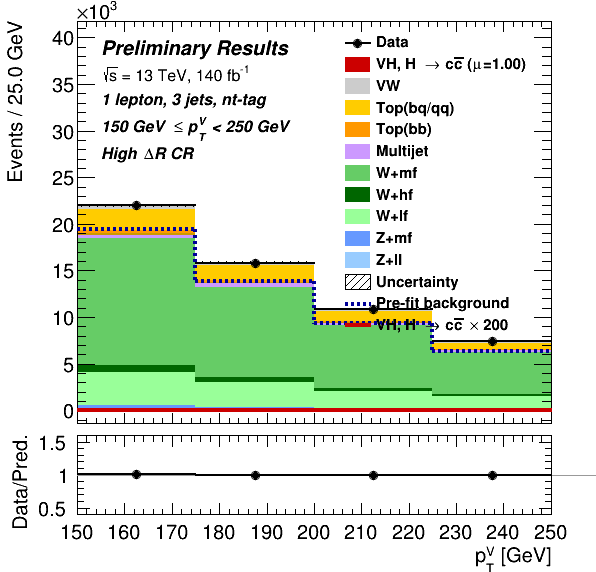
\includegraphics[width=0.32\textwidth]{Images/VH/Own_fit/postfit_VHcc/Region_distpTV_BMax250_BMin150_DCRHigh_J3_TTypent_T1_L1_Y6051_GlobalFit_conditionnal_mu1.png}
        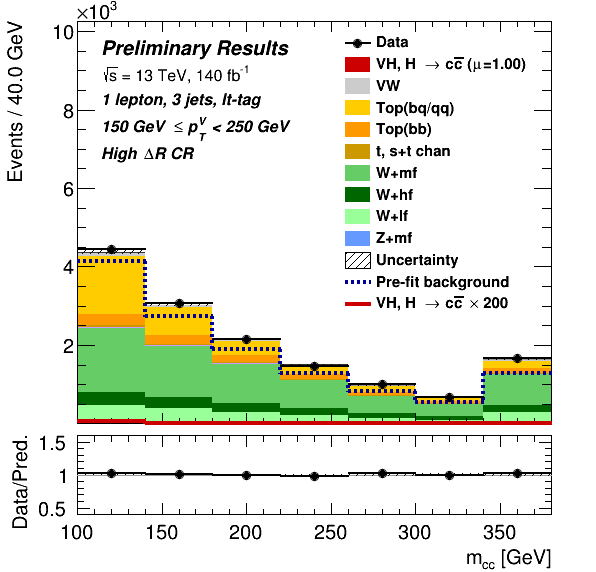
\includegraphics[width=0.32\textwidth]{Images/VH/Own_fit/postfit_VHcc/Region_distmBB_BMax250_BMin150_DCRHigh_J3_TTypelt_T2_L1_Y6051_GlobalFit_conditionnal_mu1.png}
        \includegraphics[width=0.32\textwidth]{Images/VH/Own_fit/postfit_VHcc/Region_distmBB_BMax250_BMin150_DCRHigh_J3_TTypett_T2_L1_Y6051_GlobalFit_conditionnal_mu1.png}
        \caption{150 < \ptv\ < 250 GeV.}
        \label{fig:plots_VHcc_1L_150_CRH_3J}
    \end{subfigure}
    \begin{subfigure}[b]{\textwidth}
        \centering
        \includegraphics[width=0.32\textwidth]{Images/VH/Own_fit/postfit_VHcc/Region_distpTV_BMin250_DCRHigh_J3_TTypent_T1_L1_Y6051_GlobalFit_conditionnal_mu1.png}
        \includegraphics[width=0.32\textwidth]{Images/VH/Own_fit/postfit_VHcc/Region_distmBB_BMin250_DCRHigh_J3_TTypelt_T2_L1_Y6051_GlobalFit_conditionnal_mu1.png}
        \includegraphics[width=0.32\textwidth]{Images/VH/Own_fit/postfit_VHcc/Region_distmBB_BMin250_DCRHigh_J3_TTypett_T2_L1_Y6051_GlobalFit_conditionnal_mu1.png}
        \caption{250 GeV < \ptv.}
        \label{fig:plots_VHcc_1L_250_CRH_3J}
    \end{subfigure}
    \caption{$TN$-tagged \ptv\ distributions (left) and $LT$- (centre) and $TT$-tagged (right) $H$-candidate mass distributions in the 1L \highdr\ CR 3-jet regions.}
    \label{fig:plots_VHcc_1L_CRH_3J}
\end{figure}

\vspace*{\fill} \newpage

\begin{figure}[h!]
    \centering
    \begin{subfigure}[b]{\textwidth}
        \centering
        \includegraphics[width=0.32\textwidth]{Images/VH/Own_fit/postfit_VHcc/Region_distmBB_BMax150_BMin75_DtopCRBC_J2_TTypebt_T1_L1_Y6051_GlobalFit_conditionnal_mu1.png}
        \includegraphics[width=0.32\textwidth]{Images/VH/Own_fit/postfit_VHcc/Region_distmBB_BMax250_BMin150_DtopCRBC_J2_TTypebt_T1_L1_Y6051_GlobalFit_conditionnal_mu1.png}
        \includegraphics[width=0.32\textwidth]{Images/VH/Own_fit/postfit_VHcc/Region_distmBB_BMax400_BMin250_DtopCRBC_J2_TTypebt_T1_L1_Y6051_GlobalFit_conditionnal_mu1.png}
        \caption{2-jet, [75, 150] GeV (left), [150, 250] GeV (centre), and 250 GeV $\leq$ (right) \ptv\ regions.}
        \label{fig:plots_VHcc_1L_TopCR_2J}
    \end{subfigure}
    \begin{subfigure}[b]{\textwidth}
        \centering
        \includegraphics[width=0.32\textwidth]{Images/VH/Own_fit/postfit_VHcc/Region_distmBB_BMax150_BMin75_DtopCRBC_J3_TTypebt_T1_L1_Y6051_GlobalFit_conditionnal_mu1.png}
        \includegraphics[width=0.32\textwidth]{Images/VH/Own_fit/postfit_VHcc/Region_distmBB_BMax250_BMin150_DtopCRBC_J3_TTypebt_T1_L1_Y6051_GlobalFit_conditionnal_mu1.png}
        \includegraphics[width=0.32\textwidth]{Images/VH/Own_fit/postfit_VHcc/Region_distmBB_BMax400_BMin250_DtopCRBC_J3_TTypebt_T1_L1_Y6051_GlobalFit_conditionnal_mu1.png}
        \caption{3-jet, [75, 150] GeV (left), [150, 250] GeV (centre), and 250 GeV $\leq$ (right) \ptv\ regions.}
        \label{fig:plots_VHcc_1L_TopCR_3J}
    \end{subfigure}
    \caption{$H$-candidate mass distribution in the 1L $BT$-tagged Top CRs.}
    \label{fig:plots_VHcc_1L_TopCR}
\end{figure}
\begin{figure}[h!]
    \centering
    \begin{subfigure}[b]{\textwidth}
        \centering
        \includegraphics[width=0.32\textwidth]{Images/VH/Own_fit/postfit_VHcc/Region_distpTV_BMax250_BMin150_DSR_J2_TTypeln_T1_L1_Y6051_GlobalFit_conditionnal_mu1.png}
        \includegraphics[width=0.32\textwidth]{Images/VH/Own_fit/postfit_VHcc/Region_distpTV_BMin250_DSR_J2_TTypeln_T1_L1_Y6051_GlobalFit_conditionnal_mu1.png}
        \caption{2-jet.}
        \label{fig:plots_VHcc_1L_LN_2J}
    \end{subfigure}
    \begin{subfigure}[b]{\textwidth}
        \centering
        \includegraphics[width=0.32\textwidth]{Images/VH/Own_fit/postfit_VHcc/Region_distpTV_BMax250_BMin150_DSR_J3_TTypeln_T1_L1_Y6051_GlobalFit_conditionnal_mu1.png}
        \includegraphics[width=0.32\textwidth]{Images/VH/Own_fit/postfit_VHcc/Region_distpTV_BMin250_DSR_J3_TTypeln_T1_L1_Y6051_GlobalFit_conditionnal_mu1.png}
        \caption{3-jet.}
        \label{fig:plots_VHcc_1L_SR_3J}
    \end{subfigure}
    \caption{\ptv\ distributions in the 1L $LN$-tagged $V+l$ CR [150, 250] GeV (left) and 250 GeV $\leq$ (right) \ptv\ regions.}
    \label{fig:plots_VHcc_1L_LN}
\end{figure}

\newpage

% 2L
\vspace*{\fill} 

\begin{figure}[h!]
    \centering
    \begin{subfigure}[b]{\textwidth}
        \centering
        \includegraphics[width=0.32\textwidth]{Images/VH/Own_fit/postfit_VHcc/Region_distmva_BMax150_BMin75_DSR_J2_TTypext_T2_L2_Y6051_GlobalFit_conditionnal_mu1.png}
        \includegraphics[width=0.32\textwidth]{Images/VH/Own_fit/postfit_VHcc/Region_distmva_BMax250_BMin150_DSR_J2_TTypext_T2_L2_Y6051_GlobalFit_conditionnal_mu1.png}
        \includegraphics[width=0.32\textwidth]{Images/VH/Own_fit/postfit_VHcc/Region_distmva_BMin250_DSR_J2_TTypext_T2_L2_Y6051_GlobalFit_conditionnal_mu1.png}
        \caption{2-jet, [75, 150] GeV (left), [150, 250] GeV (centre), and 250  GeV $\leq$ (right) \ptv\ regions.}
        \label{fig:plots_VHcc_2L_SR_2c_2J}
    \end{subfigure}
    \begin{subfigure}[b]{\textwidth}
        \centering
        \includegraphics[width=0.32\textwidth]{Images/VH/Own_fit/postfit_VHcc/Region_distmva_BMax150_BMin75_DSR_J3_TTypext_incJet1_T2_L2_Y6051_GlobalFit_conditionnal_mu1.png}
        \includegraphics[width=0.32\textwidth]{Images/VH/Own_fit/postfit_VHcc/Region_distmva_BMax250_BMin150_DSR_J3_TTypext_incJet1_T2_L2_Y6051_GlobalFit_conditionnal_mu1.png}
        \includegraphics[width=0.32\textwidth]{Images/VH/Own_fit/postfit_VHcc/Region_distmva_BMin250_DSR_J3_TTypext_incJet1_T2_L2_Y6051_GlobalFit_conditionnal_mu1.png}
        \caption{$\geq$3-jet, [75, 150] GeV (left), [150, 250] GeV (centre), and 250  GeV $\leq$ (right) \ptv\ regions.}
        \label{fig:plots_VHcc_2L_SR_2c_3J}
    \end{subfigure}
    \caption{\gls{bdt} distributions in the 2L 2 $c$-tagged signal regions.}
    \label{fig:plots_VHcc_2L_SR_2c}
\end{figure}
\begin{figure}[h!]
    \centering
    \begin{subfigure}[b]{\textwidth}
        \centering
        \includegraphics[width=0.32\textwidth]{Images/VH/Own_fit/postfit_VHcc/Region_distmva_BMax150_BMin75_DSR_J2_TTypent_T1_L2_Y6051_GlobalFit_conditionnal_mu1.png}
        \includegraphics[width=0.32\textwidth]{Images/VH/Own_fit/postfit_VHcc/Region_distmva_BMax250_BMin150_DSR_J2_TTypent_T1_L2_Y6051_GlobalFit_conditionnal_mu1.png}
        \includegraphics[width=0.32\textwidth]{Images/VH/Own_fit/postfit_VHcc/Region_distmva_BMin250_DSR_J2_TTypent_T1_L2_Y6051_GlobalFit_conditionnal_mu1.png}
        \caption{2-jet, [75, 150] GeV (left), [150, 250] GeV (centre), and 250  GeV $\leq$ (right) \ptv\ regions.}
        \label{fig:plots_VHcc_2L_SR_1c_2J}
    \end{subfigure}
    \begin{subfigure}[b]{\textwidth}
        \centering
        \includegraphics[width=0.32\textwidth]{Images/VH/Own_fit/postfit_VHcc/Region_distmva_BMax150_BMin75_DSR_J3_TTypent_incJet1_T1_L2_Y6051_GlobalFit_conditionnal_mu1.png}
        \includegraphics[width=0.32\textwidth]{Images/VH/Own_fit/postfit_VHcc/Region_distmva_BMax250_BMin150_DSR_J3_TTypent_incJet1_T1_L2_Y6051_GlobalFit_conditionnal_mu1.png}
        \includegraphics[width=0.32\textwidth]{Images/VH/Own_fit/postfit_VHcc/Region_distmva_BMin250_DSR_J3_TTypent_incJet1_T1_L2_Y6051_GlobalFit_conditionnal_mu1.png}
        \caption{$\geq$3-jet, [75, 150] GeV (left), [150, 250] GeV (centre), and 250  GeV $\leq$ (right) \ptv\ regions.}
        \label{fig:plots_VHcc_2L_SR_1c_3J}
    \end{subfigure}
    \caption{\gls{bdt} distributions in the 2L 1 $c$-tagged signal regions.}
    \label{fig:plots_VHcc_2L_SR_1c}
\end{figure}

\newpage
\vspace*{\fill} 


\begin{figure}[h!]
    \centering
    \begin{subfigure}[b]{\textwidth}
        \centering
        \includegraphics[width=0.32\textwidth]{Images/VH/Own_fit/postfit_VHcc/Region_distpTV_BMax150_BMin75_DCRHigh_J2_TTypent_T1_L2_Y6051_GlobalFit_conditionnal_mu1.png}
        \includegraphics[width=0.32\textwidth]{Images/VH/Own_fit/postfit_VHcc/Region_distmBB_BMax150_BMin75_DCRHigh_J2_TTypelt_T2_L2_Y6051_GlobalFit_conditionnal_mu1.png}
        \includegraphics[width=0.32\textwidth]{Images/VH/Own_fit/postfit_VHcc/Region_distmBB_BMax150_BMin75_DCRHigh_J2_TTypett_T2_L2_Y6051_GlobalFit_conditionnal_mu1.png}
        \caption{75 < \ptv\ < 150 GeV.}
        \label{fig:plots_VHcc_2L_75_CRH_2J}
    \end{subfigure}
    \begin{subfigure}[b]{\textwidth}
        \centering
        \includegraphics[width=0.32\textwidth]{Images/VH/Own_fit/postfit_VHcc/Region_distpTV_BMax250_BMin150_DCRHigh_J2_TTypent_T1_L2_Y6051_GlobalFit_conditionnal_mu1.png}
        \includegraphics[width=0.32\textwidth]{Images/VH/Own_fit/postfit_VHcc/Region_distmBB_BMax250_BMin150_DCRHigh_J2_TTypelt_T2_L2_Y6051_GlobalFit_conditionnal_mu1.png}
        \includegraphics[width=0.32\textwidth]{Images/VH/Own_fit/postfit_VHcc/Region_distmBB_BMax250_BMin150_DCRHigh_J2_TTypett_T2_L2_Y6051_GlobalFit_conditionnal_mu1.png}
        \caption{150 < \ptv\ < 250 GeV.}
        \label{fig:plots_VHcc_2L_150_CRH_2J}
    \end{subfigure}
    \begin{subfigure}[b]{\textwidth}
        \centering
        \includegraphics[width=0.32\textwidth]{Images/VH/Own_fit/postfit_VHcc/Region_distpTV_BMin250_DCRHigh_J2_TTypent_T1_L2_Y6051_GlobalFit_conditionnal_mu1.png}
        \includegraphics[width=0.32\textwidth]{Images/VH/Own_fit/postfit_VHcc/Region_distmBB_BMin250_DCRHigh_J2_TTypelt_T2_L2_Y6051_GlobalFit_conditionnal_mu1.png}
        \includegraphics[width=0.32\textwidth]{Images/VH/Own_fit/postfit_VHcc/Region_distmBB_BMin250_DCRHigh_J2_TTypett_T2_L2_Y6051_GlobalFit_conditionnal_mu1.png}
        \caption{250 GeV < \ptv.}
        \label{fig:plots_VHcc_2L_250_CRH_2J}
    \end{subfigure}
    \caption{$TN$-tagged \ptv\ distributions (left) and the $LT$- (centre) and $TT$-tagged (right) $H$-candidate mass distributions in the 2L \highdr\ CR 2-jet regions.}
    \label{fig:plots_VHcc_2L_CRH_3J}
\end{figure}

\vspace*{\fill} \newpage
\vspace*{\fill} 

\begin{figure}[h!]
    \centering
    \begin{subfigure}[b]{\textwidth}
        \centering
        \includegraphics[width=0.32\textwidth]{Images/VH/Own_fit/postfit_VHcc/Region_distpTV_BMax150_BMin75_DCRHigh_J3_TTypent_incJet1_T1_L2_Y6051_GlobalFit_conditionnal_mu1.png}
        \includegraphics[width=0.32\textwidth]{Images/VH/Own_fit/postfit_VHcc/Region_distmBB_BMax150_BMin75_DCRHigh_J3_TTypelt_incJet1_T2_L2_Y6051_GlobalFit_conditionnal_mu1.png}
        \includegraphics[width=0.32\textwidth]{Images/VH/Own_fit/postfit_VHcc/Region_distmBB_BMax150_BMin75_DCRHigh_J3_TTypett_incJet1_T2_L2_Y6051_GlobalFit_conditionnal_mu1.png}
        \caption{75 < \ptv\ < 150 GeV.}
        \label{fig:plots_VHcc_2L_75_CRH_3J}
    \end{subfigure}
    \begin{subfigure}[b]{\textwidth}
        \centering
        \includegraphics[width=0.32\textwidth]{Images/VH/Own_fit/postfit_VHcc/Region_distpTV_BMax250_BMin150_DCRHigh_J3_TTypent_incJet1_T1_L2_Y6051_GlobalFit_conditionnal_mu1.png}
        \includegraphics[width=0.32\textwidth]{Images/VH/Own_fit/postfit_VHcc/Region_distmBB_BMax250_BMin150_DCRHigh_J3_TTypelt_incJet1_T2_L2_Y6051_GlobalFit_conditionnal_mu1.png}
        \includegraphics[width=0.32\textwidth]{Images/VH/Own_fit/postfit_VHcc/Region_distmBB_BMax250_BMin150_DCRHigh_J3_TTypett_incJet1_T2_L2_Y6051_GlobalFit_conditionnal_mu1.png}
        \caption{150 < \ptv\ < 250 GeV.}
        \label{fig:plots_VHcc_2L_150_CRH_3J}
    \end{subfigure}
    \begin{subfigure}[b]{\textwidth}
        \centering
        \includegraphics[width=0.32\textwidth]{Images/VH/Own_fit/postfit_VHcc/Region_distpTV_BMin250_DCRHigh_J3_TTypent_incJet1_T1_L2_Y6051_GlobalFit_conditionnal_mu1.png}
        \includegraphics[width=0.32\textwidth]{Images/VH/Own_fit/postfit_VHcc/Region_distmBB_BMin250_DCRHigh_J3_TTypelt_incJet1_T2_L2_Y6051_GlobalFit_conditionnal_mu1.png}
        \includegraphics[width=0.32\textwidth]{Images/VH/Own_fit/postfit_VHcc/Region_distmBB_BMin250_DCRHigh_J3_TTypett_incJet1_T2_L2_Y6051_GlobalFit_conditionnal_mu1.png}
        \caption{250 GeV < \ptv.}
        \label{fig:plots_VHcc_2L_250_CRH_3J}
    \end{subfigure}
    \caption{$TN$-tagged \ptv\ distributions (left) and the $LT$- (centre) and $TT$-tagged (right) $H$-candidate mass distributions in the 2L \highdr\ CR 3-jet regions.}
    \label{fig:plots_VHcc_2L_CRH_3J}
\end{figure}

\vspace*{\fill} \newpage
\vspace*{\fill} 

\begin{figure}[h!]
    \centering
    \begin{subfigure}[b]{\textwidth}
        \centering
        \includegraphics[width=0.32\textwidth]{Images/VH/Own_fit/postfit_VHcc/Region_distpTV_BMax150_BMin75_DSR_J2_TTypeln_T1_L2_Y6051_GlobalFit_conditionnal_mu1.png}
        \includegraphics[width=0.32\textwidth]{Images/VH/Own_fit/postfit_VHcc/Region_distpTV_BMax250_BMin150_DSR_J2_TTypeln_T1_L2_Y6051_GlobalFit_conditionnal_mu1.png}
        \includegraphics[width=0.32\textwidth]{Images/VH/Own_fit/postfit_VHcc/Region_distpTV_BMin250_DSR_J2_TTypeln_T1_L2_Y6051_GlobalFit_conditionnal_mu1.png}
        \caption{2-jet, [75, 150] GeV (left), [150, 250] GeV (centre), and 250  GeV $\leq$ (right) \ptv\ regions.}
        \label{fig:plots_VHcc_2L_LN_2J}
    \end{subfigure}
    \begin{subfigure}[b]{\textwidth}
        \centering
        \includegraphics[width=0.32\textwidth]{Images/VH/Own_fit/postfit_VHcc/Region_distpTV_BMax150_BMin75_DSR_J3_TTypeln_incJet1_T1_L2_Y6051_GlobalFit_conditionnal_mu1.png}
        \includegraphics[width=0.32\textwidth]{Images/VH/Own_fit/postfit_VHcc/Region_distpTV_BMax250_BMin150_DSR_J3_TTypeln_incJet1_T1_L2_Y6051_GlobalFit_conditionnal_mu1.png}
        \includegraphics[width=0.32\textwidth]{Images/VH/Own_fit/postfit_VHcc/Region_distpTV_BMin250_DSR_J3_TTypeln_incJet1_T1_L2_Y6051_GlobalFit_conditionnal_mu1.png}
        \caption{$\geq$3-jet, [75, 150] GeV (left), [150, 250] GeV (centre), and 250  GeV $\leq$ (right) \ptv\ regions.}
        \label{fig:plots_VHcc_2L_LN_3J}
    \end{subfigure}
    \caption{\ptv\ distributions in the 2L $LN$-tagged $V+l$ CRs.}
    \label{fig:plots_VHcc_2L_LN}
\end{figure}

\begin{figure}[h!]
    \centering
    \begin{subfigure}[b]{\textwidth}
        \centering
        \includegraphics[width=0.32\textwidth]{Images/VH/Own_fit/postfit_VHcc/Region_distpTV_BMax150_BMin75_Dtopemucr_J2_TTypeta_T2_L2_Y6051_GlobalFit_conditionnal_mu1.png}
        \includegraphics[width=0.32\textwidth]{Images/VH/Own_fit/postfit_VHcc/Region_distpTV_BMax250_BMin150_Dtopemucr_J2_TTypeta_T2_L2_Y6051_GlobalFit_conditionnal_mu1.png}
        \includegraphics[width=0.32\textwidth]{Images/VH/Own_fit/postfit_VHcc/Region_distpTV_BMax400_BMin250_Dtopemucr_J2_TTypeta_T2_L2_Y6051_GlobalFit_conditionnal_mu1.png}
        \caption{2-jet, [75, 150] GeV (left), [150, 250] GeV (centre), and 250  GeV $\leq$ (right) \ptv\ regions.}
        \label{fig:plots_VHcc_2L_topCRemu_2J}
    \end{subfigure}
    \begin{subfigure}[b]{\textwidth}
        \centering
        \includegraphics[width=0.32\textwidth]{Images/VH/Own_fit/postfit_VHcc/Region_distpTV_BMax150_BMin75_Dtopemucr_J3_TTypeta_T2_L2_Y6051_GlobalFit_conditionnal_mu1.png}
        \includegraphics[width=0.32\textwidth]{Images/VH/Own_fit/postfit_VHcc/Region_distpTV_BMax250_BMin150_Dtopemucr_J3_TTypeta_T2_L2_Y6051_GlobalFit_conditionnal_mu1.png}
        \includegraphics[width=0.32\textwidth]{Images/VH/Own_fit/postfit_VHcc/Region_distpTV_BMax400_BMin250_Dtopemucr_J3_TTypeta_T2_L2_Y6051_GlobalFit_conditionnal_mu1.png}
        \caption{$\geq$3-jet, [75, 150] GeV (left), [150, 250] GeV (centre), and 250  GeV $\leq$ (right) \ptv\ regions.}
        \label{fig:plots_VHcc_2L_topCRemu_3J}
    \end{subfigure}
    \caption{\ptv\ distributions in the 2L Top $e\mu$ CR with $\geq$1 $T$-tagged regions.}
    \label{fig:plots_VHcc_2L_topCRemu}
\end{figure}
